\documentclass{standalone}
\usepackage{tikz}
\usepackage{ctex,siunitx}
\usepackage{tkz-euclide}
\usepackage{amsmath}
\usetikzlibrary{patterns, calc}
\usetikzlibrary {decorations.pathmorphing, decorations.pathreplacing, decorations.shapes,}
\begin{document}
\small
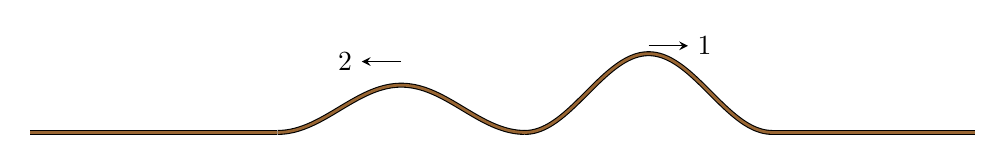
\begin{tikzpicture}[>=stealth, scale=1.0,samples=200]
  % \useasboundingbox(0,-0.6)rectangle(12,0.7);
  \draw [double=brown!80!black,double distance=1pt, domain=0:pi]  plot (\x,-0.5);
  \draw [double=brown!80!black,double distance=1pt, domain=2*pi:3*pi]  plot (\x,{-0.5*cos(2*\x r)});
  % \draw [double=brown!80!black,double distance=1pt, domain=1.5*pi:2.5*pi]  plot (\x,-0.5);
  \draw [double=brown!80!black,double distance=1pt, domain=pi:2.0*pi]  plot (\x,{-0.3*cos(2*\x r)-0.2});
  \draw [double=brown!80!black,double distance=1pt, domain=3.0*pi:12]  plot (\x,-0.5);
  \draw[thin,->](2.5*pi,0.6)--++(0.5,0)node[right]{1};
  \draw[thin,->](1.5*pi,0.4)--++(-0.5,0)node[left]{2};
\end{tikzpicture}
\end{document}